\documentclass[12pt]{article}
%\usepackage{arev}
\usepackage[utf8]{inputenc}
%\usepackage{cmbright}
%\usepackage{sansmathfonts}
\usepackage[T1]{fontenc}
\usepackage[sfdefault,scaled=.85]{FiraSans}
\usepackage{newtxsf}
%\renewcommand*\familydefault{\sfdefault}
\usepackage{amsfonts}
%\usepackage{amsthm}
\usepackage{amsmath}
\usepackage{amssymb}
%\usepackage{mathabx}
\usepackage{mathrsfs}
\usepackage{graphicx}
\usepackage{multicol}
\usepackage{array}
\usepackage{tasks}
\usepackage{mathrsfs}
\usepackage[dvipsnames*,svgnames,x11names,table,xcdraw]{xcolor}
\usepackage[margin=2cm]{geometry}
\usepackage{tikz}
\usetikzlibrary{automata,arrows,cd}
\usepackage{etoolbox,expl3,environ}
\usepackage{enumerate}
\usepackage{setspace}
\usepackage{pdflscape}
\usepackage{tcolorbox}
\usepackage{fancyhdr}
\usepackage{listings} 
\usepackage{minted}
\usepackage{hyperref}
\usepackage[hybrid, hashEnumerators,smartEllipses]{markdown}
\usepackage{titlesec}
\usepackage{booktabs}
\usepackage{tabularx}

\newcommand{\tabitem}{~~\llap{\textbullet}~~}
\titlelabel{\thetitle.\quad}

\setlength{\parindent}{0cm}
\spacing{1}
\usemintedstyle{monokai}
\setminted[python]{escapeinside =||,
                    mathescape = true, 
                    frame = lines,
                    framesep = 2mm,
                    baselinestretch = 1.2,
                    bgcolor = black,
                    fontsize = \footnotesize,
                    linenos}

%\theoremstyle{definition}
%\newtheorem*{definition}{Definición}

\NewDocumentCommand{\myrule}{O{1pt} O{2pt} O{black}}{%
  \par\nobreak % don't break a page here
  \kern\the\prevdepth % don't take into account the depth of the preceding line
  \kern#2 % space before the rule
  {\color{#3}\hrule height #1 width\hsize} % the rule
  \kern#2 % space after the rule
  \nointerlineskip % no additional space after the rule
}

\pagestyle{fancy}
\fancyhf{}
\lhead{\textbf{Almacenes y Minería de Datos 2024-1 \\ Tarea 01. Información Estratégica}}
\rhead{\textbf{PostgresandoesoSQLazos}}
\headheight 35pt
\renewcommand{\headrulewidth}{0.5pt}



\newcommand{\om}{\omega}
\newcommand{\lam}{\lambda}
\newcommand{\be}{\beta}
\newcommand{\al}{\alpha}
\newcommand{\ro}{\rho}

\newcommand{\N}{\mathbb{N}}
\newcommand{\Z}{\mathbb{Z}}
\newcommand{\C}{\mathbb{C}}
\newcommand{\R}{\mathbb{R}}

\newcommand{\ex}{\exists}
\newcommand{\fa}{\forall}
\newcommand{\nex}{\nexists}
\newcommand{\vn}{\varnothing}
\newcommand{\sbq}{\subseteq}
\newcommand{\spq}{\supseteq}
\newcommand{\w}{\widehat{\delta}}
\newcommand{\la}{\Longrightarrow}

\newcommand{\ov}[1]{\overline{#1}}

\newenvironment{sol}{\paragraph{Solución.}}{\hfill$\square$}
\newenvironment{dem}{\paragraph{Demostración.}}{\hfill$\square$}

\definecolor{azul}{RGB}{218, 232, 252}



\begin{document}

\begin{titlepage}
\begin{center}
\textbf{\LARGE Universidad Nacional Autónoma de México}\\[0.5cm] 
\textbf{\Large Facultad de Ciencias, 2024 - 1}\\[0.2cm]
% \vspace{20pt}\includegraphics[width=5cm]{algo.jpeg}\\
% \par
\vspace{20pt}
\textbf{\Large Almacenes y Minería de Datos}\\
\vspace{3pt}
\myrule[1pt][7pt]
\textbf{\LARGE  Tarea 01. Información Estratégica}\\
\vspace{15pt}
\textbf{\LARGE PostgresandoesoSQLazos}\\
\myrule[1pt][7pt]
\vspace{35pt}
\begin{figure}[htbp]
  \centering
  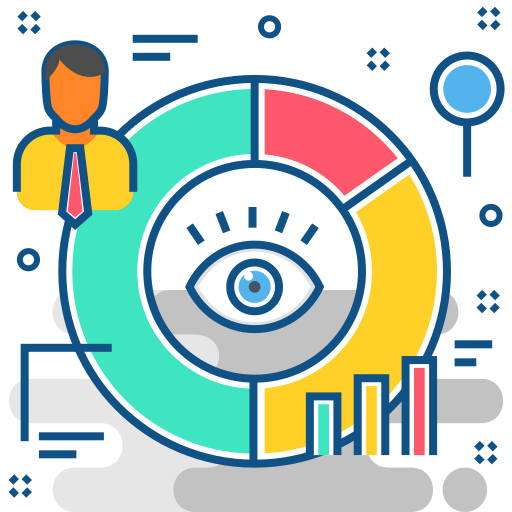
\includegraphics[scale=0.8]{../img/business.png}
\end{figure}
\textbf{\Large Integrantes}\\
\vspace{15pt}


\begin{tabular}{c c}
    Adrian Aguilera Moreno & 421005200 \\
    Marco Antonio Rivera Silva & 318183583 \\
    Sebastían Alejandro Gutiérrez Medina & 318287021 \\
    Israel Hernández Dorantes & 318206604 \\
    Alejandra Ortega García & 420002495 \\
\end{tabular}

\end{center}
\par
\end{titlepage}


\section*{Resumen de Artículo}

    \subsection{Prehistoria Relacional}

        Los sistemas de bases de datos relacionales surgieron en la década de 1970 como respuesta a los crecientes costos de implementación y mantenimiento de sistemas complejos. La principal problemática que abordaron fue la necesidad de que los programadores, que eran costosos, tuvieran que reescribir gran parte del software cada vez que la estructura o la organización física de la BD cambiaba. Para solucionar esto, los sistemas de bases de datos relacionales ocultaron la organización la BD a la y utilizaron un lenguaje declarativo para describir los datos, permitiendo a los programadores enfocarse en lo que deseaban sin preocuparse por los detalles de optimización y acceso a la BD.\\

        Estos sistemas tuvieron un gran éxito en empresas y centros de datos, generando un mercado multimillonario en ingresos por licencias. Sin embargo, en las décadas siguientes, surgieron dos tendencias relacionadas: el aumento de la funcionalidad de los sistemas de bases de datos y la falta de necesidad de muchas de estas características para la mayoría de las aplicaciones. Esto condujo a una creciente complejidad en su administración, requiriendo especialistas en bases de datos, a pesar de que muchos programas solo utilizaban una fracción de las características disponibles. La pregunta que se plantea es si existe una mejor manera de abordar esta complejidad y simplificar la gestión de bases de datos.\\

    \subsection{La Nueva Frontera}

        En 1998, los principales investigadores en bases de datos notaron que los SMBD se estaban volviendo demasiado complejos y que la configuración y gestión automatizada se estaban volviendo esenciales. Dos años después, Surajit Chaudhuri y Gerhard Weikum propusieron una reestructuración radical de la arquitectura de los SMBD, abogando por hacerlos más modulares y utilizar bloques de construcción basados en componentes simples en lugar de enfoques complejos.\\

        Michael Stonebraker también argumentó que el enfoque único de los SMBD relacionales ya no es adecuado para todas las necesidades de gestión de datos. Señaló que los proveedores de bases de datos relacionales han estado proporcionando la ilusión de que un sistema de gestión de bases de datos relacionales (RDBMS) es la respuesta a cualquier necesidad de gestión de datos, pero esta idea se vuelve inadecuada a medida que surgen nuevas necesidades de datos.\\
        
        Se mencionan varios ejemplos de nuevas problemáticas en la gestión de datos, como data warehousing (almacenamiento de datos), servicios de directorio, búsqueda en la web, almacenamiento en caché en dispositivos móviles, gestión de XML y procesamiento de transmisiones en tiempo real. Estos ejemplos muestran cómo las necesidades de gestión de datos están evolucionando hacia aplicaciones específicas que requieren enfoques diferentes a los sistemas de bases de datos relacionales tradicionales.

    \subsection{Soluciones Flexibles}

        Los sistemas de bases de datos relacionales tradicionales están diseñados principalmente para satisfacer cargas de trabajo de procesamiento de transacciones en línea (OLTP). Estas cargas de trabajo se caracterizan por consultas \textit{ad hoc}, un tráfico significativo de escritura y la necesidad de garantías transaccionales e integridad. Sin embargo, muchas de las aplicaciones actuales son dominadas por lectura , y algunas aplicaciones de \textit{streaming} ni siquiera aprovechan datos persistentes, sino que utilizan un lenguaje de consulta similar a SQL. Además, pocas de estas aplicaciones requieren garantías transaccionales y los datos que manejan no tienen una estructura inherentemente relacional.\\

        Para abordar estas cambiantes necesidades de gestión de datos, se destaca la importancia de la flexibilidad. Se presentan tres enfoques para lograrlo. El primero consiste en que cada aplicación construya su propio servicio de almacenamiento de datos, pero esta opción es impráctica en la mayoría de las aplicaciones. El segundo enfoque es proporcionar una variedad de opciones de gestión de datos, cada una diseñada para una clase específica de aplicaciones. El ultimo enfoque es desarrollar un motor de almacenamiento más configurable que pueda adaptarse a los requisitos de aplicaciones individuales, aunque esto requerirá que los desarrolladores comprendan las opciones de configuración.\\
        
        Se argumenta que la solución emergente en el mercado es tener unos pocos sistemas de almacenamiento razonablemente configurables, cada uno útil para una amplia clase de aplicaciones. Es importante que dos propiedades fundamentales que una solución debe tener para abordar las diversas necesidades de las aplicaciones son la modularidad y la configurabilidad. La modularidad permite a los programas utilizar solo las partes necesarias del sistema de gestión de datos, evitando que paguen por funcionalidad no utilizada en términos de tamaño, complejidad o costo. La configurabilidad permite adaptar el sistema a diferentes entornos operativos y hardware.

    \subsection{Modularidad}

    Algunos coinciden en que la arquitectura de las bases de datos necesitan una renovación pues la arquitectura DBMS monolítica convencional no es tan simple como para adaptarse a las demandas actuales, en especifico se refieren a implementar módulos pequeños simples y reusables que mejoren la productividad.

    El concepto de arquitectura basada en componentes se puede ampliar para incluir varios otros aspectos del diseño de bases de datos: control de concurrencia, transacciones, registros y alta disponibilidad.

    Se mencionan varios ejemplos de como SQL podría ser mejorado y crear familias de lenguajes mucho más enriquecidas que puedan adaptarse mejor a las necesidades actuales. \\

    Se propone también que las transacciones a pesar de no es necesario tratarlas de forma separada, deberían de separarse, ya que algunas no utilizan un sistema de registros (lo cual deriva en que también el sistema de registros pueda usarse en otro contexto que no sean las transacciones), sin embargo la decisión de separar las transacciones siempre deberá ser decisión del diseñador. \\

    Otra de las ventajas de la arquitectura modular, es mejorar la capacidad de proporcionar la disponibilidad de los datos, pues como sabemos, hay datos que son tan valiosos, que simplemente al tenerlos inactivos se está perdiendo mucho (tanto en recursos, como en otros factores) y esto es motivo suficiente para justificar la innovación en la arquitectura, pues los sistemas monolíticos no proporcionan estas ventajas. Por otro lado, en el aspecto de aplicaciones también se destaca la arquitectura modular, pues permite generar aplicaciones, más simples y ligeras, pues simplemente se utilizaría lo necesario y siempre permite la opción de extender o agregar módulos para cubrir más necesidades.

    \subsection{Configurabilidad}

    La configurabilidad es otra parte importante, ya que mientras la modularidad se encarga de dar estructura, la configurabilidad es en esencia un mecanismo en tiempo de ejecución. \\

    Es importante mantener buenas opciones de configuración, esto debido a la gran cantidad de posibilidades que pueden tener las combinaciones de componentes (incluso solo una combinación), y sumando a esto la gran cantidad de entornos en los que se pueden desempeñar nuestros sistemas.

    De igual forma se debe de hacer configurable para la gran cantidad de software que existe en el mercado, ya que incluso podría causar problemas en cuanto a la compatibilidad de los componentes de la estructura de nuestro sistema. \\

    Se especifica que la base de datos no debe de tomar decisiones sobre protocolos de red, pues en caso de que algún componente externo, tenga sus preferencias o protocolos especiales de red, deberán de ser compatibles con la base (sin que esta interfiera).

    Por último la configurabilidad también radica en los datos de la aplicación. Hay tres puntos principales de diseño con respecto a los datos: la agrupación física, el mecanismo de indexación y la estructura interna de los elementos de la base de datos. Las bases se pueden centrar en configurar partes especificas de estos 3 puntos. Por lo tanto un motor configurable es una gran ayuda para determinar la estructura interna de los datos.

    

    \subsection{Nuevo Estilo de Base de Datos Para Nuevos Problemas}

    Podemos decir que la necesidad de sistemas de gestión de bases de datos convencionales no ha desaparecido, pues muchos de los problemas actuales requieren un sistema de base de datos que sea configurable (y aún más en el futuro). Con el tiempo aprendemos a seleccionar las herramientas adecuadas para hacer un trabajo y de igual forma lo hacemos con las bases de datos. \\
    
    Necesitamos trabajar de modo que podamos reconocer que existen opciones en la gestión de datos y debemos seleccionar la herramienta adecuada para realizar el trabajo de la forma más eficiente, sólida y sencilla posible

    
\newpage

\section*{Ensayos}

\subsection*{Adrián Aguilera Moreno}

En la actualidad el alto crecimiento de las poblaciones ha implicado un alto desarrollo en tecnologías, que a su vez genera un alto impacto en la cantidad de datos generados en el mundo. Uno de los grandes deseos de muchas empresas es controlar estos datos para apoyar en ellos decisiones que acometen a sus respectivas empresas o negocios, sin embargo el tener estos grandes cúmulos de datos no significan que a su vez sean provechosos.\newline

En los años 80's hubo grandes necesidades de mejorar la manera en que los programadores administraban los datos, pues por cada cambio en la organización o en la estructura de los datos, debían programar nuevamente estas maneras de almacenar y gestionar su información. Durante la misma época, algunas instituciones desarrollaron nuevas maneras de abordar estos problemas, la solución fue la creación de los Sistemas Relacionales Manejadores de Datos. Este desarrollo tuvo cómo impacto el traer una gran demanda por muchas empresas, sin embargo, lo que se les vendían eran paquetes monolíticos\footnote{Esto es, paquetes con software que no necesariamente necesitaban, pero iba incluido.} por lo que los precios eran altos.\newline

En los próximos años el interés por este tipo de gestión relacional de los datos creció, sin embargo, la problemática de tener que adquirir grandes paquetes de software a la vez seguía prevaleciendo, algunos investigadores y personas del medio decidieron desarrollar nuevas maneras de gestionar la información de manera relacional que a su vez combatiera las problemáticas no abordados en sus inicios. A partir de aquí se crea y populariza el lenguaje SQL. Con la llegada de SQL y la modularización del software se crea una gran demanda en el mercado y \textit{una mejor gestión de los datos}.\newline

Sin embargo, esta manera de gestionar datos era rígida al momento de configurar las bases de datos correspondientes y le daban poca libertad al desarrollador o especialista. Cómo alternativa para garantizar flexibilidad de configurabilidad de las bases de datos y así se dota al desarrollador de herramientas que le permitían gestionar y almacenar información de manera personalizada.\newline

Ante todo esto, se empezó a pensar ¿Podemos sacarle provecho a los datos que no tengan una estructura cómo la que se manejaba hasta el momento? En este punto se empeso a administrar información en formato \textbf{XML} por ejemplo, sin embargo muchos archivos no comparten un mismo formato y non comparten en especial el formato del lenguaje SQL, que desde entonces y hasta el momento es uno de los más utilizados en el ramo.\newline

Tiempo después, y para darle solución ha este tipo de problemáticas, se crea los almacenes de datos cómo una manera de mejora continua en la organización, gestión y almacenamiento de los mismos. Sin embargo, este tipo de mejora vuelve a tener cierta problemática que se había logrado erradicar, como lo es la venta por paquetes. Pero si vuelven a cometer estos errores ¿Por qué son viables? La respuesta es muy sencilla, a partir de la creación de modularización se han creado paquetes pequeños y específicos llamados módulos que logran agrupar ciertas herramientas que logran ser suficientes para pequeñas empresas, dándole la opción de  adquirir módulos más grandes a empresas que así lo requieran.\newpage

\subsection*{Marco Antonio Rivera Silva}

Las bases de datos fueron una gran herramienta que ayudó desde el momento de su creación a solucionar múltiples problemas. Sin embargo con el paso del tiempo (y como toda herramienta en el mundo de la computación), las bases de datos tuvieron que evolucionar poco a poco para extender su campo de aplicación. Por desgracia, actualmente el uso de nuestros sistemas ha quedado \textit{estancado} en los sistemas monolíticos pues por lo general ayudan a solucionar casi todos nuestros problemas. Esto llevo a que se comenzaran a desarrollar nuevas formas de hacer bases de datos, en este caso una arquitectura basada en módulos. \\

Está nueva forma de estructurar las bases de datos, aún no está completamente perfeccionada, pero nos muestra algunos de los frutos de la modularidad y las posibles configuraciones que puede tener alguno de nuestros sistemas (destacando que en nuestros días la variedad de software y hardware pueden crear muchísimas combinaciones). Pudimos ver como se han realizado diversos métodos para mejorar tanto las capacidades de nuestros lenguajes de consulta, como los motores y estructuras de datos que emplean nuestras bases de datos. \\

Es importante destacar que la implementación de este nuevo tipo de arquitectura siempre estará bajo la consideración los desarrolladores, pues utilizarán las mejores herramientas y configuraciones para resolver problemas específicos, pues como sabemos no todas los sistemas sirven para todos los casos, estos deben de ser optimizados cuidadosamente. \\

Todo esto también nos ha llevado a pensar en el futuro, pues podemos ver un crecimiento exponencial en cuanto al uso de los datos que tenemos en la sociedad actual y por lo tanto, es obvio que en algún momento nuestras soluciones dejarán de ser las más efectivas (si es que no lo son ya). Por lo que optimizar poco a poco nuestros sistemas a las nuevas problemáticas no es una opción, sino una obligación. \\

Considero que el articulo plante muy buenos puntos sobre la mesa en cuanto a la importancia sobre las alternativas a nuestros sistemas actuales, en especial en la parte donde plantea el nuevo estilo de las bases de datos para futuros problemas, ya que nos hace tomar conciencia de la importancia de las decisiones del desarrollador tanto en la parte del software, como del hardware y de las posibles problematicas que desee resolver.

\newpage
\subsection*{Sebastián Alejandro Gutiérrez Medina}

    Cuando las bases de datos relacionales surgieron hace ya varias décadas, estas lograron resolver varios problemas con el manejo de datos que habían surgido, sin embargo, con el tiempo este modelo se ha vuelto insuficiente con el creciente volumen de datos y necesidades de procesamiento de dichos datos, aunque cada SMBD ha implementado diversas herramientas y funcionalidades para resolver algunos de estos problemas la verdad es que no todos los casos de uso necesitan todas esas herramientas, pues aunque útiles, no tienden a ser sencillas de utilizar, por lo que es necesario que una BD pueda se independiente de algunas de estas herramientas y funciones, logrando así una modularidad del sistema.\\

    Siendo este el caso es importante para un desarrollador poder identificar cuales son sus necesidades y al mismo tiempo conocer que herramientas y funciones son necesarias para cubrir sus requerimientos, ya que no podemos continuar con la mentalidad de que una herramienta puede hacerlo todo, por lo que es necesario mantenerse actualizado con los nuevos desarrollos en las BD.\\

    Por otro lado, es indispensable denotar que aunque una herramienta o función puede ser útil para cubrir alguna necesidad del sistema, esto va a depender del grado de integración que podamos darle a dicha herramienta o función y esto va a depender en gran medida del grado de configurabilidad que el SMBD pueda brindarnos para cada herramienta o función.\\

    Estos son los que yo considero los puntos que el articulo \textit{Beyond Relational Databases} trata de transmitir, pues es importante reconocer que es necesario crear diferentes estilos de bases de datos para poder enfrentar los nuevos problemas que estan surgiendo en los tiempos actuales.\\

\newpage
\subsection*{Israel Hernández Dorantes}

En la actualidad existen muchas computadoras, tabletas y teléfonos móviles que ofrecen nuevas aplicaciones y servicios; y los desarrolladores de software siguen creando más servicios que hace muchos años era imposible. Y para estos servicios ha surgido la \textit{necesidad de crear funciones de almacenamiento y recuperación de datos integradas}; pues esto es un aspecto fundamental para todas las aplicaciones y servicios que usamos a diario. Y para ello se han utilizado las bases de datos relacionales para la gestión de datos en las últimas tres décadas hasta ahora, o eso lo veremos.\\

En los años 1970's surgieron las \textbf{bases de datos relacionales}, las cuales ocultaban la organización física de las bases de datos de las aplicaciones proporcionando una vista lógica de los datos; y se utilizaba un \textit{lenguaje declarativo} que permitía describir los datos de interés en una consulta (query) específica. Y esto permitió que los programadores no tuvieran que volver a reescribir el código cada vez que la organización de la bases de datos cambiaba.\\
Pero durante los años de 1990's se encontraron nuevos problemas que surgieron por la gestión de los datos, los cuales son el \textbf{almacenamiento de datos}, \textbf{servicio de directorio}, \textbf{búsqueda web}, \textbf{almacenamiento caché de dispositivos móviles}, \textbf{gestión XML}, \textbf{procesamiento de flujo}, entre otros. Y por ello existen varias formas de ofrecer flexibilidad en el ambiente cambiante de los datos; una consiste en un enfoque de \textit{regreso a lo básico} en el que cada aplicación crea su propio servicio de almacenamiento de datos; otra forma es proporcionar una mezcla de opciones de manejo de datos; y otra forma es produciendo un motor de almacenamiento más configurable. Y estas soluciones deben de cumplir con la \textit{modularidad} y \textit{configurabilidad}.\\

La \textit{modularidad} consiste en una herramienta poderosa que se ha utilizado para administrar el tamaño y complejidad de las aplicaciones y sistemas, y permitiendo también la capacidad de que las aplicaciones y el manejo de datos interactúen. Los tipos de arquitectura basados en la modularidad han permitido a los desarrolladores poder excluir funcionalidades que no necesitan y que no son pertenecientes del proveedor de la base de datos.\\

La \textit{configurabilidad} es la segunda propiedad de un sistema de bases de datos flexible, la cual consiste en qué tan bien un sistema se puede adaptar a su entorno y a las necesidades de la aplicación. Y hasta hoy la configurabilidad ha girado en torno a adaptarse al entorno de hardware y software de la aplicación.\\

Finalmente, podemos concluir que los sistemas de bases de datos \textit{antiguos} resuelven problemas \textit{antiguos}, y los sistemas de bases de datos \textit{nuevos} resuelven problemas \textit{nuevos}; pues muchos de los problemas actuales necesitan de un sistema de bases de datos configurables. Aunque como programadores debemos de escoger la herramienta adecuada para realizar un determinado trabajo de la manara más eficiente y simple posible.


\newpage




\subsection*{Alejandra Ortega García}

El surgimiento de nuevas tecnologías da pie al incremento de la demanda de datos, es decir, la necesidad de que servicios de mensajería, multimedia, búsqueda por localización, etc.,  puedan almacenar y recuperar datos fiables y de manera rápida. La solución más popular a esta problemática, al menos en las tres últimas décadas, fueron las bases de datos relacionales, RDBMS. Con las  bases de datos relacionales los desarrolladores agilizan la implementación y mantenimiento de sistemas complejos; ocultan la organización física y únicamente proporcionan una vista lógica de los datos y utilizan un lenguaje declarativo (SQL) para poder obtener información. Sin embargo, contar con RDBMS se volvió costoso, pues los proveedores incrementaron la funcionalidad de la bases de datos. . ¿Existe alguna otra forma de solucionar esto?\\


A medida de que el manejo de base de datos se volvía cada vez más compleja, los investigadores llegaron a la conclusión de que la configuración y gestión  automatizada se estaban transformando en algo esencial. Propusieron la idea de modularizar los sistemas manejadores de bases de datos y ampliar nuestra perspectiva sobre el manejo de datos, considerando sistemas más simples basados en componentes.\\


Como existen aplicaciones de distintos tipos, debemos centrarnos en soluciones flexibles que puedan adaptarse a las necesidades de cada una de ellas. De acuerdo con el artículo \textit{Beyond Relational Databases}, hay varias maneras de obtener flexibilidad. Por ejemplo, que cada aplicación implementa su propio servicio de almacenamiento de datos, ofrecer múltiples opciones para el manejo de datos o contar con un motor de almacenamiento que sea más configurable. \\


En este entorno tecnológico en constante cambio, la flexibilidad se convierte en un elemento esencial para garantizar la eficiencia y la adaptabilidad en el manejo de datos. Por lo tanto, la búsqueda de soluciones flexibles y modulares se presenta como una respuesta inteligente para satisfacer las necesidades cambiantes de las aplicaciones en el futuro.

\newpage
\section{Conceptos Generales}
\begin{enumerate}[a.]
\item Describe las principales características del enfoque de bases de datos y contrástalo con el enfoque basado en archivos. ¿En qué casos tendría sentido utilizar el enfoque de archivos?


Las principales características del enfoque de bases de datos son que se deben de \textbf{almacenar datos interrelacionados} en un 
\textbf{contexto o semántica} con un \textbf{objetivo en específico}.


Puede \textbf{almacenar una enorme cantidad de información}, mientras que en los archivos tienen más limitantes en cuanto al tamaño de datos que puede almacenar.
    

Debe de haber un \textbf{intermediario entre el usuario y la base de datos}, que es el sistema manejador de bases de datos, el cual debe de definir (tipos, restricciones y estructuras), construir (almacenar los datos en algún medio de almacenamiento controlado por el SABD) y compartir (permitir el acceso a más usuarios),  mientras que en el enfoque basado en archivos no existe este intermediario aquellos que tienen acceso con el archivo lo tienen de manera directa en una copia del archivo fragmentando la realidad.
    

Los datos deben poder ser \textbf{actualizados y deben de estar protegidos}, por otro lado con un enfoque de archivos no aseguran una
protección de los datos, ya que, al compartir los archivos no es posible que den una buena protección, incluso podría llegar a ser nula. 
    

Su objetivo principal es proporcionar una \textbf{forma de almacenar y recuperar la información de manera práctica y eficiente}, el enfoque basado en archivos almacena y recupera información, pero no lo hace de manera práctica ni eficiente.
    
Por lo tanto un caso en el que \textbf{tendría sentido usar archivos} es cuando no hay una gran cantidad de datos a almacenar o en casos en los que sólo existe un usuario que accede, manipula y actualiza
los datos, pues no habría necesidad de presentar una clase de restricción.

\item Indica las diferencias (emplea una tabla para contrastarlas) en cuanto a cómo se representan los datos entre una hoja de cálculo y una base de datos relacional.

\begin{table}[ht]
    \centering
    \begin{tabularx}{\textwidth}{lX X}
        \toprule
        \textbf{Aspecto} & \textbf{Hojas de Cálculo} & \textbf{Bases de Datos Relacionales} \\
        \midrule
        Estructura de Datos & Bidimensional (filas y columnas) en celdas individuales. & Tablas con filas y columnas; permite relaciones entre tablas. \\
        Relaciones de Datos & Referencias de celda y fórmulas. & Relaciones mediante llaves primarias y foráneas. \\
        Integridad de Datos & Menos rigurosas; propensas a errores humanos. & Mantenimiento de la integridad a través de reglas y restricciones. \\
        Capacidad de Consulta & Adecuadas para análisis y cálculos pequeños. & Permiten consultas avanzadas y optimizadas con SQL. \\
        Escalabilidad & Menos eficientes con grandes volúmenes de datos. & Manejan grandes volúmenes de datos y escalan mejor. \\
        \bottomrule
    \end{tabularx}

\end{table}

\newpage
\item ¿Qué ventajas y desventajas encuentras al trabajar con una hoja de cálculo?

Ventajas:
\begin{itemize}
    \item Permiten una mejor \textit{apreciación} de los datos que se estén guardando pues estos se muestran de una manera organizada.

    \item Permiten poder realizar cálculos matemáticos de forma automatizada con los datos que se guarden.

    \item Muestran un historial de los cambios que se hayan realizado de los datos en las hojas, para así poder revertir cambios no deseados.

    \item Permiten crear funciones y fórmulas que realicen tareas automatizadas para así ahorrar tiempo en el manejo de los datos.

    
\end{itemize}

Desventajas:
\begin{itemize}

    \item Son de tamaño limitado, por lo cual no serán una buena opción para guardar grandes cantidades de datos.

    \item Si se trata de un registro muy grande, el ingreso de los datos requerirán de mayor tiempo y esfuerzo.

    \item Si existe algún error en las fórmulas o funciones que se hayan creado, todos los datos que hayan sido procesados serán incorrectos.

    \item Entre más grande sean las hojas de cálculo, serán más difíciles de escalar para implementaciones futuras.
    


    
\end{itemize}


\item ¿Qué ventajas y desventajas encuentras al trabajar con una base de datos?

Ventajas:
\begin{itemize}
    \item Ofrecen acceder a los datos de una forma rápida y 
    eficiente.
    \item Al existir el sistema manejador de bases de datos evita la fragmentación de la realidad, existe un sólo lugar donde los datos están almacenados.
    \item Puede almacenar grandes cantidades de información.
    \item Permite a varios usuarios visualizar los datos que les interesen.
\end{itemize}

Desventajas:
\begin{itemize}
    \item No cualquier persona puede crear, mantener o actualizar una base de datos, por lo menos no de manera eficiente.
    \item Su proceso de construcción es difícil.
    \item No son accesibles para todos, para muchos resulta más económico, de momento, usar otros métodos de almacenamiento y
    manejo de datos.
\end{itemize}



\item ¿Qué es un sistema OLTP y cuáles son sus características principales?

Un sistema OLTP (sistema de procesamiento de transacciones en línea) es un tipo de sistema diseñado para procesar transacciones en línea en tiempo real, el cual consiste en una arquitectura de tres niveles:
\begin{itemize}
    \item Nivel de presentación: Es donde la transacción se origina a través de una interacción humana o generada por el sistema.
    
    \item Nivel de lógica de negocio: Es donde se verifica  la transacción y se garantiza que todos los datos necesarios para completar la transacción estén disponibles.

    \item Nivel de almacén de datos: Es donde se almacena la transacción y todos los datos relacionados con ella.
    
\end{itemize}

Y sus principales características son:
\begin{itemize}
    \item \textbf{Alto rendimiento y tiempo de respuesta corto}: Proporcionan respuestas rápidas a las solicitudes para poder mantener la productividad de los usuarios empresariales y satisfacer las expectativas de los clientes.
    
    \item \textbf{Concurrencia}: Garantiza que puedan tener muchos usuarios que intentan acceder a los mismos datos al mismo tiempo.

   \item \textbf{Disponibilidad}: El sistema se encuentra siempre disponible y listo para aceptar transacciones.

   \item \textbf{Seguridad}: Proporcionan una alta seguridad debido a que se almacenan datos de transacciones confidenciales de los clientes.

   \item \textbf{Recuperación}: Poseen la capacidad de recuperarse en caso de fallo de hardware o software.

   \item \textbf{Escala}: Pueden ampliar y reducir al instante la gestión del volumen de transacciones en tiempo real y ejecutar transacciones de forma simultánea.

    
\end{itemize}



\item ¿Qué entiendes por información estratégica? Para una cadena de supermercados, indica cinco tipos de objetivos estratégicos.

La \textbf{información estratégica} es aquella que ayuda a las organizaciones a tomar decisiones y a planificar acciones que les permitan alcanzar sus objetivos de negocio.

\begin{enumerate}[1.]
    \item \textbf{Expansión y crecimiento:} La expansión geográfica de la cadena, abriendo nuevas sucursales en ubicaciones estratégicas para aumentar la presencia en el mercado y atraer a nuevos clientes.

    \item \textbf{ Optimización de la cadena de suministro:} Mejorar la eficiencia y la gestión de la cadena de suministro asegura un flujo constante de productos a las sucursales.

    \item \textbf{Innovación tecnológica:} Integrar tecnologías como una aplicación móvil, análisis de datos y soluciones de pago innovadoras puede ayudar a la cadena de supermercados a mantenerse al día.
    
    \item \textbf{Mejora de la experiencia del cliente:} Proporcionar un ambiente agradable en las sucursales, ofrecer un excelente servicio al cliente.

    \item \textbf{Desarrollo de marcas y productos propios:} La creación y promoción de marcas y productos propios de la cadena de supermercados puede aumentar los beneficios.
\end{enumerate}

\item Investiga qué papel juegan los analistas de bases de datos, diseñadores y desarrolladores de bases de datos en la construcción de un sistema de bases de datos.

\begin{itemize}
    \item \textbf{Analista: } Evalúa el diseño de las bases de datos; reúne, organiza e interpreta la información estadística basada en los datos de la base de datos.

    \item \textbf{Diseñador: } Se encarga de identificar los datos que se van a almacenar en la base de datos y de elegir las estructuras adecuadas para representar y almacenar estos datos. Además, tienen la responsabilidad de comunicarse con todos los posibles usuarios de la base de datos para entender sus requisitos y crear un diseño que satisfaga estos requisitos.

    \item \textbf{Desarrollador: } Son los principales responsables de la creación e implementación de bases de datos. Determinan el mejor SMBD para un usuario concreto, además de probar los programas de bases de datos para comprobar su eficacia, rendimiento, solucionar y corregir problemas.


\end{itemize}

\item Imagina que eres el director de TI de una cadena de minoristas a nivel nacional. Redacta un informe al presidente ejecutivo explicando las oportunidades, beneficios y ventajas que se pueden tener con información estratégica que se tenga fácilmente disponible.\newline

La información estratégica, en esta empresa, puede ser un punto de diferenciación con empresas representativas en el ramo. La información estratégica permitirá tener claro lo que sucede en cada uno de los departamentos, si está información no se extrae de manera clara y estratégica podría llevar a la empresa a tomar decisiones no tan correctas y no tan fundamentadas cómo las que se toman con un información filtrada.\newline

Es necesario obtener una información histórica para predecir y tomar decisiones a futuro. La función de la información estratégica es obtener datos procesados valiosos que puedan generar decisiones que guíen todas las posibles situaciones a mejores soluciones. Dicho lo anterior, es evidente que el hacer uso y obtener este tipo de información beneficia de manera importante las futuras decisiones de la empresa.

\item ¿Cómo se define la calidad de datos? ¿Por qué consideras que es importante en el entorno actual?

La \textbf{calidad de datos} se refiere a la integridad y exactitud de los datos, así como a su capacidad para proporcionar información precisa y valiosa que respalde la toma de decisiones, el análisis u otras operaciones. 

A medida que las organizaciones dependen cada vez más de los datos para impulsar sus operaciones y estrategias, asegurar que los datos sean confiables, precisos y relevantes se convierte en una \textbf{prioridad clave} para mantener la eficiencia, la competitividad y la toma de decisiones en este entorno.


\item Indica al menos seis características que debe tener un entorno informático para proporcionar información estratégica.\newline

Su función primordial no es apoyar la automatización de procesos operativos ni proporcionar información para apoyar la toma de decisiones. A continuación se en listan algunas características:
\begin{itemize}
\item Buen diseño.
\item Facilidad de uso.
\item Flexibilidad en recursos.
\item Mantenimiento automático de los registros.
\item Apoyo en toma de decisiones críticas.
\item Mantener el anonimato en informaciones no relevantes.
\end{itemize}

\item ¿Qué son los datos? ¿Cómo se relacionan los datos en tu vida profesional? ¿Cómo contribuyes a la
generación de datos?\newline

Los datos son información concreta sobre hechos, elementos, etc., que permite estudiarlos, analizarlos o conocerlos. Los datos funcionan en nuestro día a día como estudiantes, para recabar información y poder formular conocimiento. Al realizar, esta tarea por ejemplo, y actividades diarías como estudiantes generamos nuevos datos concretos y partículares que generan conocimientos para cada uno de nosotros.

\item ¿Qué es información? ¿Cómo se relaciona la información con tu vida profesional?

Podemos definir primero la \textbf{información} como \textit{un conjunto de datos organizados, procesados y analizados que brindan conocimiento, contexto y comprensión sobre un tema particular}; por lo cual la \textbf{información} nos va a permitir poder realizar un conjunto de habilidades y actividades que son esenciales para la \textbf{vida profesional}, como lo son la toma de decisiones (bien argumentadas), resolución de problemas previamente analizados, comunicación efectiva para la transmisión de información clara, entre otros; los cuales son aspectos fundamentales para poder desarrollarse y mejorar en el ámbito profesional.


\item ¿Qué es conocimiento? ¿Cómo se relaciona el conocimiento con tu vida profesional?

Primero podemos definir el conocimiento como \textit{el resultado que se obtiene de experimentación, razonamiento y aprendizaje}; por lo cual el \textit{conocimiento} nos va a permitir desarrollar habilidades, resolver problemas y tener una mejor comunicación, los cuales son aspectos fundamentales para la \textbf{vida profesional}, pues esto nos permite desarrollarnos en el ámbito profesional consiguiendo las habilidades suficientes para realizar los trabajos que se piden, tomar decisiones informadas, adaptarse a nuevas situaciones y tecnologías, y proporcionar innovaciones que beneficien a un algún grupo de personas. 


\item Investiga qué es el Gobierno de Datos y por qué consideras que es importante para la generación de
información estratégica.\newline

El gobierno de datos permite disponer de una visión integral de la información facilitando una responsabilidad compartida en las decisiones. Uno de los objetivos principales del gobierno de datos es lograr un entendimiento común del dato. El gobierno de datos es imprescindible en todas las empresas de todos los sectores, ya que los datos se han ido convirtiendo en su recurso más valioso al avanzar en su transformación digital. Un dato puede significar un número, una letra, un signo ortográfico o cualquier símbolo que represente una cantidad, una medida, una palabra o una descripción. La importancia de los datos está en su capacidad de asociarse dentro de un contexto para convertirse en información.

\item ¿Qué métodos has utilizado para convertir datos en información?
\begin{itemize}
\item Filtración. Eliminar filas que no cumplan criterios específicos
\item Inserción. Agregar elementos nuevos para encontrar información de manera progresiva.
\item Actualización. Actualización de datos equivocos.
\item Eliminación. Eliminación de información obsoleta, cambio en la organización.
\item Ordenación. Reorganizar los datos en un orden específico.
\item Unión. Combinar tablas basadas en una columna común. Combina tablas con las mismas columnas.
\end{itemize}
\end{enumerate}
\end{document}
